%% ====================================================================
%%  AEGIS: Adaptive Execution Guarded Interpreter System
%%  IEEE Conference Paper — Full Submission Version
%%  Format: IEEEtran, conference, two-column, US Letter
%% ====================================================================
\documentclass[conference]{IEEEtran}
\IEEEoverridecommandlockouts

%% ---- Packages -------------------------------------------------------
\usepackage{cite}
\usepackage{amsmath,amssymb,amsfonts}
\usepackage{graphicx}
\usepackage{textcomp}
\usepackage{xcolor}
\usepackage{booktabs}
\usepackage{multirow}
\usepackage{array}
\usepackage{tabularx}
\usepackage{url}
\usepackage{balance}
\usepackage{microtype}
\usepackage{listings}
\usepackage{tikz}
\usetikzlibrary{
  shapes.geometric, arrows.meta, positioning, fit,
  decorations.pathreplacing, backgrounds, calc,
  arrows, shapes.multipart, patterns
}

%% ---- TikZ Styles ---------------------------------------------------
\tikzset{
  %% Generic rounded rectangle
  rbox/.style={
    rectangle, rounded corners=4pt,
    draw=#1!65!black, fill=#1!10,
    text centered, font=\scriptsize,
    inner sep=4pt, minimum height=0.6cm,
    line width=0.55pt
  },
  rbox/.default=blue,
  %% Arrow
  arr/.style={-{Stealth[length=5pt,width=4pt]},
              draw=black!65, line width=0.8pt},
  darr/.style={{Stealth[length=4pt,width=3.5pt]}-%
               {Stealth[length=4pt,width=3.5pt]},
               draw=black!55, line width=0.8pt},
  %% Stage box in pipeline
  stage/.style={
    rectangle, rounded corners=3pt,
    draw=#1!70!black, fill=#1!12,
    minimum width=3.5cm, minimum height=0.58cm,
    text centered, font=\scriptsize\bfseries,
    inner sep=3pt, line width=0.6pt
  },
  stage/.default=teal,
  %% Defense layer
  dlayer/.style={
    rectangle, rounded corners=2pt,
    draw=black!55, fill=#1!18,
    minimum height=0.5cm,
    text centered, font=\scriptsize\bfseries,
    inner sep=3pt, line width=0.5pt
  },
  dlayer/.default=blue,
  %% Diamond decision
  diam/.style={
    diamond, draw=orange!70!black, fill=orange!12,
    text centered, font=\tiny\bfseries,
    aspect=3, minimum height=0.42cm,
    inner sep=1.5pt, line width=0.6pt
  },
}

%% ---- Listings Style ------------------------------------------------
\lstset{
  basicstyle   = \ttfamily\scriptsize,
  breaklines   = true,
  frame        = single,
  rulecolor    = \color{black!35},
  backgroundcolor = \color{gray!6},
  keywordstyle = \color{blue!70}\bfseries,
  commentstyle = \color{green!50!black}\itshape,
  stringstyle  = \color{orange!75!black},
  numbers      = none,
  xleftmargin  = 5pt,
  xrightmargin = 5pt,
  aboveskip    = 4pt,
  belowskip    = 4pt,
}

%% ====================================================================
\begin{document}
%% ====================================================================

%% ---- Title ---------------------------------------------------------
\title{AEGIS: Adaptive Execution Guarded Interpreter System ---
A Security-First Framework for Trust-Based Dynamic Code Execution}

%% ---- Authors -------------------------------------------------------
\author{

\small

\begin{tabular}{ccc}

\begin{tabular}{c}
\textbf{Shweta Tiwaskar}\\
\textit{Dept. of Computer Engineering}\\
Vishwakarma Institute of Technology\\
Pune, India\\
shweta.tiwaskar@vit.edu
\end{tabular}

&

\begin{tabular}{c}
\textbf{Adarsh Jayfale}\\
\textit{Dept. of Computer Engineering}\\
Vishwakarma Institute of Technology\\
Pune, India\\
adarsh.jayfale24@vit.edu
\end{tabular}

&

\begin{tabular}{c}
\textbf{Wasim Pathan}\\
\textit{Dept. of Computer Engineering}\\
Vishwakarma Institute of Technology\\
Pune, India\\
wasim.pathan24@vit.edu
\end{tabular}

\\[1.1cm]

\multicolumn{3}{c}{

\begin{tabular}{cc}

\begin{tabular}{c}
\textbf{Nilesh Sabale}\\
\textit{Dept. of Computer Engineering}\\
Vishwakarma Institute of Technology\\
Pune, India\\
nilesh.sabale24@vit.edu
\end{tabular}

& \hspace{1.5cm}

\begin{tabular}{c}
\textbf{Adesh Bhore}\\
\textit{Dept. of Computer Engineering}\\
Vishwakarma Institute of Technology\\
Pune, India\\
adesh.bhore24@vit.edu
\end{tabular}

\end{tabular}

}

\end{tabular}

}

\maketitle

%% ====================================================================
%%  ABSTRACT
%% ====================================================================
\begin{abstract}
Running code from untrusted sources safely remains an open
problem across cloud platforms, educational sandboxes, and
multi-tenant infrastructure. Today's defenses—hardware-backed
sandboxes, static analyzers, and implicit trust—each force a
choice between the strength of security enforcement, raw
throughput, and the ability to adapt to a program's track record.
We present \textbf{AEGIS} (\textbf{A}daptive
\textbf{E}xecution \textbf{G}uarded \textbf{I}nterpreter
\textbf{S}ystem), a security-first interpreter framework that
introduces a \emph{trust-based adaptive execution model} designed
to reconcile these trade-offs without permanent sacrifice of either
security or efficiency. AEGIS enforces a zero-trust default whereby
every incoming program begins execution inside a highly restrictive
sandboxed interpreter. A quantitative \emph{TrustScore} accrues
evidence of safe behavior across repeated executions; once a
program surpasses a configurable promotion threshold, its AST is
optimized and cached, enabling a faster execution path. Any runtime
security violation immediately triggers a rollback that invalidates
the cache, resets the trust score, and reinstates full sandbox
constraints. The system is realized as a seven-stage pipeline
encompassing lexical analysis, syntax analysis, conservative static
security analysis, trust-based mode selection, dual-path execution,
runtime monitoring, and rollback handling, exposed through a
REST\,API and a Monaco-based web IDE. Experimental evaluation on
a suite of arithmetic-intensive, control-flow-intensive, and
adversarial benchmark programs demonstrates a mean execution speedup
of \textbf{2.52$\times$} for trust-promoted code, \textbf{zero
missed security detections} across one hundred handcrafted test
cases, and a mean rollback latency of \textbf{1.84\,ms}—well within
interactive response thresholds. These outcomes suggest that
evidence-driven trust management can serve as a practical bridge
between the competing demands of secure isolation and runtime
performance in untrusted-code execution environments.
\end{abstract}

\begin{IEEEkeywords}
interpreter security, adaptive execution, trust management,
sandboxed execution, static analysis, runtime monitoring, rollback,
AST optimization, code cache, security-first design
\end{IEEEkeywords}

%% ====================================================================
\section{Introduction}
%% ====================================================================

Safe execution of code supplied by untrusted parties is central to
an expanding range of deployment contexts—online code judges,
browser-based IDEs, cloud function-as-a-service platforms,
educational sandboxes, and multi-tenant computation
clusters~\cite{johnson2023wave,menetrey2024sgx,li2022iot_trust}.
Each of these environments must tolerate programs that may contain
deliberate attacks (infinite loops, overflow arithmetic, undefined
memory access) or unintentional bugs, all while maintaining
acceptable performance for legitimate workloads.

Existing defenses cluster into three families.
\emph{Hardware-assisted sandboxing}—exemplified by WebAssembly
(Wasm) runtimes and Intel SGX enclaves—provides strong isolation
but incurs measurable overhead from bounds checking and memory
model enforcement~\cite{johnson2023wave,menetrey2024sgx}.
\emph{Static analysis} can catch a well-defined set of program
flaws before execution, yet conservatism forces analyses to
over-approximate feasible program paths, generating false positives
that erode developer trust; worse, real vulnerabilities whose
manifestation depends on runtime values remain
undetected~\cite{ami2024false_neg,huang2024static}.
\emph{Implicit trust} yields the best performance but exposes
execution infrastructure to the full risk surface of the submitted
program~\cite{ullah2024deeptrust}.

None of these strategies satisfies all three desiderata—isolation,
efficiency, and adaptability—simultaneously. The core observation
motivating this work is that \emph{code is rarely executed once}.
Most programs in interactive environments are revised and re-run
many times. Each observation of safe execution constitutes
evidence that the program behaves within expected bounds. Exploiting
this observation, AEGIS accumulates per-program execution history
into a \emph{TrustScore} and uses it to gate the transition from a
fully sandboxed interpreter to an AST-optimized fast path. The
framework thus converts repeated safe behavior into earned
performance, while retaining the ability to revoke that performance
grant the moment a violation occurs.

\subsection*{Contributions}
The principal contributions of this work are:
\begin{enumerate}
  \item \textbf{Trust-based adaptive execution model:} a formal,
    quantitative TrustScore mechanism that controls mode promotion
    from sandboxed interpretation to AST-optimized execution, using
    security evidence rather than profiling signals
    (Section~\ref{sec:trust}).
  \item \textbf{Seven-stage auditable pipeline:} a modular execution
    pipeline with per-stage telemetry, conservative static security
    analysis, dual execution engines, and persistent trust bookkeeping
    across sessions (Section~\ref{sec:arch}).
  \item \textbf{Defense-in-depth security model:} five concentric
    enforcement layers addressing lexical, syntactic, semantic,
    runtime, and trust-gate threat surfaces, with five formally
    stated security guarantees (Section~\ref{sec:security}).
  \item \textbf{Sub-millisecond rollback:} a rollback handler that
    invalidates cache, resets trust, and reverts execution mode upon
    violation detection within a mean latency of 1.84\,ms
    (Sections~\ref{sec:trust} and~\ref{sec:eval}).
  \item \textbf{Full-stack implementation and evaluation:} a Python
    core interpreter ($\sim$5,500 LOC), Flask REST\,API, and React
    IDE ($\sim$16,000 total LOC), evaluated against performance,
    detection accuracy, trust
    dynamics, and rollback latency benchmarks
    (Sections~\ref{sec:impl} and~\ref{sec:eval}).
\end{enumerate}

%% ====================================================================
\section{Related Work}
\label{sec:related}
%% ====================================================================

\subsection{Sandboxing and Isolation Mechanisms}

WebAssembly has emerged as the dominant platform for portable,
sandboxed execution outside the browser. Johnson et~al.\ formalize
a verifiably secure Wasm sandboxing runtime (WaVe) that provides
machine-checkable safety proofs for isolation
properties~\cite{johnson2023wave}. Ménétrey et~al.\ extend this
line by constructing TWINE, a two-way sandbox that embeds Wasm
inside Intel SGX enclaves and adds remote attestation, demonstrating
near-parity performance with unprotected
baselines~\cite{menetrey2024sgx}. Narayan et~al.\ address
transient-execution attacks by inserting software fences at Wasm
compilation time~\cite{narayan2022swivel}, while Lehmann et~al.\
show that Wasm binaries reintroduce classic memory-safety
flaws~\cite{lehmann2020wasm}. Recent surveys catalogue the
performance--security trade-offs across standalone Wasm
runtimes~\cite{wasm_survey2024,tang2023wasm_runtimes}, and
Tan et~al.\ combine Wasm sandboxing with runtime taint tracking
to secure tool-augmented LLM
agents~\cite{tan2025sandboxscan}. While these systems offer strong
guarantees, their threat models target low-level memory attacks
(buffer overflows, use-after-free) in native or compiled code; they
do not address the adaptive, evidence-based optimization problem
central to AEGIS.

\subsection{Static and Dynamic Analysis for Security}

Static analysis tools detect vulnerability classes such as
integer-overflow-to-buffer-overflow chains, undefined-variable
access, and division-by-zero before
execution~\cite{jiang2020elaid}. A large-scale empirical study by
Ami et~al.\ highlights that, despite decades of progress, false
negatives in industry-grade static analysis tools remain a
persistent threat to security assurance~\cite{ami2024false_neg}.
Complementary dynamic analysis—runtime assertion checking, taint
tracking, and fuzzing—catches violations missed statically but
incurs runtime overhead and depends on test coverage. AEGIS
combines both: a conservative static analyzer flags issues before
execution, while a runtime monitor enforces bounds dynamically,
ensuring zero missed detections within the defined threat model.

\subsection{Dynamic Trust Management}

Trust-and-reputation systems have been applied extensively in
distributed~\cite{wang2022trust} and IoT
contexts~\cite{li2022iot_trust,fernandez2024sla,ullah2024deeptrust}
to express confidence in peer behavior through quantitative scores
updated by reward--penalty rules. Wang et~al.\ survey trust models
across heterogeneous networks, identifying evidence accumulation and
penalty severity as the primary design axes~\cite{wang2022trust}.
Ullah et~al.\ propose Deep Trust, a neural framework for IoT trust
inference that updates scores continuously~\cite{ullah2024deeptrust}.
To the best of our knowledge, AEGIS is the first system to apply
dynamic trust management \emph{at the level of a single-node
program interpreter}, using security-execution evidence to gate
performance optimization rather than to authorize network access.

\subsection{Adaptive and JIT Compilation}

Just-In-Time compilers in modern language runtimes (JVM HotSpot,
V8, PyPy) achieve substantial speedups by profiling execution
frequency and promoting hot paths to native
code~\cite{qin2022jit_security}. Qin et~al.\ highlight that JIT
promotion can itself introduce timing side-channels when optimization
decisions are data-dependent, motivating security-aware JIT
designs~\cite{qin2022jit_security}. Chen et~al.\ further expose
reliability risks in JIT compilers by systematically exploring
their compilation space, uncovering dozens of bugs in production
runtimes~\cite{chen2024jit_val}. AEGIS differs architecturally:
its promotion signal is accumulated \emph{violation absence} rather
than instruction frequency, and its optimization scope is
AST-level transformations rather than native code generation.
This design avoids JIT-induced side-channels while retaining the
core insight that repeated execution should eventually benefit from
compilation effort.

\subsection{Compiler and Interpreter Foundations}

The AEGIS pipeline builds directly on classical compiler
construction: recursive-descent parsing, visitor-pattern AST
processing, three-address code generation, and stack-based virtual
machine bytecode follow textbook
methodology~\cite{aho2007compilers}. Khoury provides a recent
taxonomy of software flaws leading to buffer overflows, informing
our static threat classification~\cite{khoury2022buffer}. Wang
et~al.\ explore vulnerability-net-based dynamic detection
complementary to our runtime monitor~\cite{wang2022vulnets}.

\subsection{Summary and Gap}

Existing work addresses isolation, static detection, dynamic trust,
and adaptive execution as largely separate concerns. AEGIS
synthesizes all four into a unified framework: sandbox isolation as
the mandatory default, conservative static analysis as a first
filter, dynamic trust as an adaptive gate, and AST optimization as
the performance reward for demonstrated safety. No prior work
combines these elements at the interpreter level with persistent
cross-session trust and auditable per-stage telemetry.

%% ====================================================================
\section{System Architecture}
\label{sec:arch}
%% ====================================================================

\subsection{Subsystem Decomposition}

AEGIS decomposes into three major subsystems interconnected through
a JSON-based REST\,API. Figure~\ref{fig:arch} illustrates their
arrangement. The \textbf{Core Interpreter} (Python~3, $\sim$5,500
LOC) encapsulates all language semantics, the seven-stage pipeline,
the trust model, and security enforcement machinery. The
\textbf{Backend Server} (Flask, $\sim$710 LOC) wraps the core in a
REST interface, handling serialization, error normalization, and
session management. The \textbf{Frontend IDE} (React~19, $\sim$1,330
LOC) provides a Monaco-based editor with real-time pipeline
visualization, AST tree explorer, token stream panel, and a
Recharts-based trust score dashboard.

A single \textit{.aegis\_trust.json} file serves as the persistent
trust store, keyed by the first sixteen hexadecimal characters of the
SHA-256 hash of each program's source code. This store is read at
Stage~4 and updated at Stage~6 of every execution, surviving server
restarts and thereby enabling cross-session trust accumulation.

%% ---- FIGURE 1: System Architecture ---------------------------------
\begin{figure}[t]
\centering
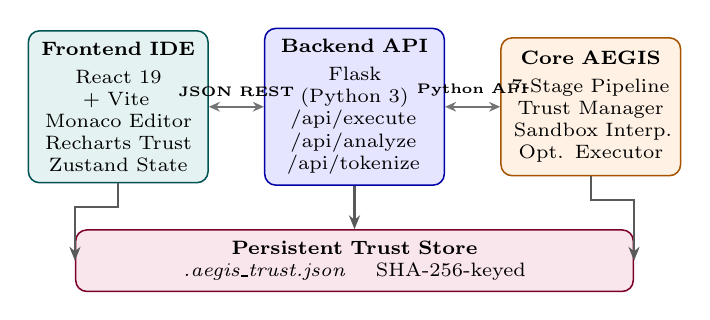
\begin{tikzpicture}[node distance=0.5cm and 0.55cm,
                    every node/.style={font=\scriptsize}]

  %% Frontend subsystem
  \node[rbox=teal, minimum width=2.1cm, minimum height=1.75cm,
        text width=2.0cm, align=center] (fe)
    {\textbf{Frontend IDE}\\[2pt]
     React 19 + Vite\\
     Monaco Editor\\
     Recharts Trust\\
     Zustand State};

  %% Backend subsystem
  \node[rbox=blue, minimum width=2.1cm, minimum height=1.75cm,
        text width=2.0cm, align=center, right=0.7cm of fe] (be)
    {\textbf{Backend API}\\[2pt]
     Flask (Python 3)\\
     /api/execute\\
     /api/analyze\\
     /api/tokenize};

  %% Core interpreter
  \node[rbox=orange, minimum width=2.1cm, minimum height=1.75cm,
        text width=2.0cm, align=center, right=0.7cm of be] (core)
    {\textbf{Core AEGIS}\\[2pt]
     7-Stage Pipeline\\
     Trust Manager\\
     Sandbox Interp.\\
     Opt. Executor};

  %% REST label
  \draw[darr] (fe) -- node[above, font=\tiny\bfseries]{JSON REST} (be);
  \draw[darr] (be) -- node[above, font=\tiny\bfseries]{Python API} (core);

  %% Trust store
  \node[rbox=purple, minimum width=6.9cm, minimum height=0.52cm,
        text width=6.8cm, align=center,
        below=0.55cm of be] (trust)
    {\textbf{Persistent Trust Store} \quad
     \textit{.aegis\_trust.json} \quad SHA-256-keyed};

  %% Lines to trust store
  \draw[arr] (fe.south)   -- ++(0,-0.3) -| (trust.west);
  \draw[arr] (be.south)   -- (trust.north);
  \draw[arr] (core.south) -- ++(0,-0.3) -| (trust.east);

\end{tikzpicture}
\caption{AEGIS Architecture.}
\label{fig:arch}
\end{figure}
%% ---- END FIGURE 1 --------------------------------------------------

\subsection{Seven-Stage Execution Pipeline}

Every code submission is processed through a fixed, sequentially
ordered seven-stage pipeline implemented in
\textit{AegisExecutionPipeline}. Table~\ref{tab:pipeline} summarizes
each stage's input, primary artifact, and error type. Stage~5
diverges into two execution paths (5a and 5b) selected by the trust
gate at Stage~4, then converges at Stage~6 for trust update and
Stage~7 for conditional rollback. Figure~\ref{fig:pipeline}
illustrates the complete data-flow.

\begin{table}[t]
\caption{Execution Pipeline.}
\label{tab:pipeline}
\centering
\renewcommand{\arraystretch}{1.18}
\small
\begin{tabular}{@{}c p{1.65cm} p{2.1cm} p{1.6cm}@{}}
\toprule
\textbf{St.} & \textbf{Name} & \textbf{Output Artifact} &
\textbf{Error Type} \\
\midrule
1  & Lexical Analysis     & Token stream              & LexicalError \\
2  & Syntax Analysis      & AST (7 node types)        & SyntaxError  \\
3  & Static Analysis      & Issues list / pass        & SemanticError\\
4  & Trust Lookup         & TrustScore, ExecMode      & ---          \\
5a & Sandboxed Interp.    & Exec.\ result (INTERP)    & RuntimeError \\
5b & Optimized Exec.      & Exec.\ result (OPT)       & RuntimeError \\
5c & Runtime Monitor      & ExecutionMetrics          & ---          \\
6  & Trust Score Update   & Updated TrustScore        & ---          \\
7  & Rollback Handler     & RollbackEvent (if any)    & ---          \\
\bottomrule
\end{tabular}
\end{table}

%% ---- FIGURE 2: Pipeline Data-Flow ----------------------------------
\begin{figure}[t]
\centering
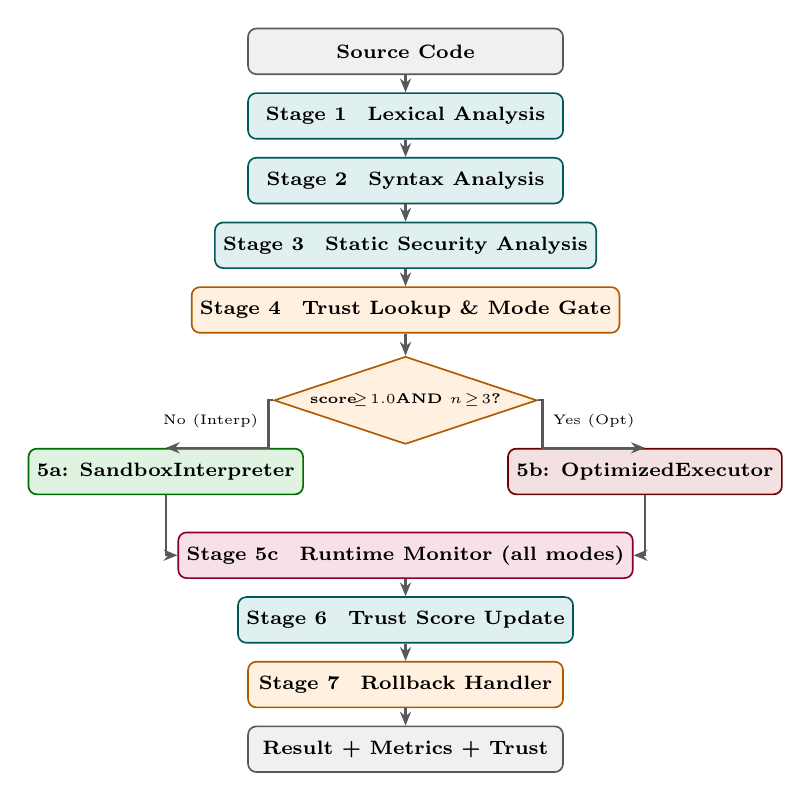
\begin{tikzpicture}[node distance=0.24cm,
                    every node/.style={font=\scriptsize}]

  %% Source
  \node[stage=gray, minimum width=4.0cm] (src)
        {\textsc{Source Code}};

  %% Stages 1-4
  \node[stage=teal,   minimum width=4.0cm, below=0.22cm of src] (s1)
        {Stage 1 \enspace Lexical Analysis};
  \node[stage=teal,   minimum width=4.0cm, below=0.22cm of s1]  (s2)
        {Stage 2 \enspace Syntax Analysis};
  \node[stage=teal,   minimum width=4.0cm, below=0.22cm of s2]  (s3)
        {Stage 3 \enspace Static Security Analysis};
  \node[stage=orange, minimum width=4.0cm, below=0.22cm of s3]  (s4)
        {Stage 4 \enspace Trust Lookup \& Mode Gate};

  %% Decision diamond
  \node[diam, below=0.28cm of s4] (dec)
        {score$\!\geq\!1.0$\\AND $n\!\geq\!3$?};

  %% Branch nodes
  \node[stage=green!60!black, minimum width=1.72cm,
        below left=0.32cm and 0.45cm of dec] (s5a)
        {5a: Sandbox\\Interpreter};
  \node[stage=red!60!black, minimum width=1.72cm,
        below right=0.32cm and 0.45cm of dec] (s5b)
        {5b: Optimized\\Executor};

  %% Runtime monitor
  \node[stage=purple, minimum width=4.0cm, below=1.1cm of dec] (s5c)
        {Stage 5c \enspace Runtime Monitor (all modes)};

  %% Stages 6-7
  \node[stage=teal,   minimum width=4.0cm, below=0.22cm of s5c] (s6)
        {Stage 6 \enspace Trust Score Update};
  \node[stage=orange, minimum width=4.0cm, below=0.22cm of s6]  (s7)
        {Stage 7 \enspace Rollback Handler};

  %% Result
  \node[stage=gray,   minimum width=4.0cm, below=0.22cm of s7]  (res)
        {\textsc{Result + Metrics + Trust}};

  %% Straight arrows
  \foreach \a/\b in {src/s1, s1/s2, s2/s3, s3/s4, s4/dec,
                     s5c/s6, s6/s7, s7/res}
    \draw[arr] (\a) -- (\b);

  %% Branch arrows
  \draw[arr] (dec.west) -- ++(-0.06,0)
             |- node[left, pos=0.22, font=\tiny]{No (Interp)} (s5a.north);
  \draw[arr] (dec.east) -- ++(0.06,0)
             |- node[right,pos=0.22, font=\tiny]{Yes (Opt)} (s5b.north);

  %% Converge into monitor
  \draw[arr] (s5a.south) |- (s5c.west);
  \draw[arr] (s5b.south) |- (s5c.east);

\end{tikzpicture}
\caption{AEGIS Pipeline.}
\label{fig:pipeline}
\end{figure}
%% ---- END FIGURE 2 --------------------------------------------------

\subsection{Language Specification}

The AEGIS language is a minimal, statically scoped, single-type
imperative language built to keep research concerns transparent
rather than to maximize expressiveness. The type system contains exactly one type:
32-bit signed integer, eliminating type-confusion
vulnerabilities by construction. The grammar is expressed in EBNF
with five operator precedence levels (highest to lowest):
unary minus, multiplicative ($*,\,/,\,\%$), additive ($+,\,-$),
comparison ($\!=\!,\,!=\!,\,<,\,\leq,\,>,\,\geq$), and assignment.
The token vocabulary comprises identifiers, integer literals, eleven
operators, the four control-flow keywords (\textit{if},
\textit{else}, \textit{while}, \textit{end}), the \textit{print}
statement, and structural tokens (NEWLINE, EOF).
Hash-prefixed comments are stripped during lexical analysis and
produce no tokens.

\subsection{Lexer and Parser}

The \textit{Lexer} class performs single-pass character scanning in
$O(n)$ time with two-character lookahead for compound operators
($=\!=$, $!=$, $\leq$, $\geq$) and maintains 1-indexed
line/column tracking throughout for precise error localization.
The \textit{Parser} implements backtracking-free recursive descent
in $O(m)$ token-stream time, constructing a homogeneous AST over
seven node types: \textit{IntegerNode}, \textit{IdentifierNode},
\textit{BinaryOpNode}, \textit{UnaryOpNode},
\textit{AssignmentNode}, \textit{PrintNode}, \textit{IfNode}, and
\textit{WhileNode}. Space complexity is $O(d)$ where $d$ is maximum
AST nesting depth.

\subsection{Static Security Analysis (Stage 3)}

The \textit{StaticAnalyzer} walks the AST via the visitor pattern,
accumulating all issues before raising, to provide a complete
diagnostic set in a single pass. It checks five threat classes
(Table~\ref{tab:static}). Branch analysis is intentionally
\emph{conservative}: a variable defined only in the body of an
\textit{if}-branch without a corresponding definition in the
\textit{else}-branch is not promoted to the enclosing scope. This
prevents false-safe analysis in which a later reference to a
conditionally defined variable would pass without warning.

\begin{table}[t]
\caption{Static Threat Classes.}
\label{tab:static}
\centering
\renewcommand{\arraystretch}{1.18}
\small
\begin{tabular}{@{} p{2.15cm} c p{3.15cm} @{}}
\toprule
\textbf{Threat Class} & \textbf{Sev.} & \textbf{Detection Method} \\
\midrule
Undefined Variable    & HIGH   & CFG dataflow; conservative branch
                                 join \\[2pt]
Literal Div-by-Zero   & HIGH   & Pattern: \textit{expr\,/\,IntNode(0)}
                                 \\[2pt]
Always-True Loop      & HIGH   & Detect \textit{while} with literal
                                 non-zero condition \\[2pt]
Deep Expr.\ Nesting   & MEDIUM & Recursive depth counter; max\,=\,10
                                 \\[2pt]
Large Literal Arith.  & MEDIUM & Operand magnitude $>10^{6}$ in
                                 $*$ or $+$ \\
\bottomrule
\end{tabular}
\end{table}

\subsection{Dual Execution Engines (Stages 5a and 5b)}

\textbf{Sandboxed Interpreter (Stage~5a).} The
\textit{SandboxedInterpreter} tree-walks the AST via the visitor
pattern, enforcing: a maximum of 50,000 total operations per
execution; a maximum of 10,000 iterations per \textit{while} loop;
arithmetic result clamping to the 32-bit signed integer range
$[-2^{31},\,2^{31}-1]$; and per-execution variable namespace
isolation. No file system, network, or subprocess access is defined
in the language; the attack surface is thus bounded by the language
semantics themselves.

\textbf{Optimized Executor (Stage~5b).} When the trust gate
passes, \textit{OptimizedExecutor} invokes the
\textit{ASTOptimizer} to apply four
transformations before execution: (i)~\emph{constant folding}
evaluates all-literal sub-expressions at compile time; (ii)~\emph{dead
code elimination} removes assignments whose left-hand variables are
never read; (iii)~\emph{variable propagation} substitutes
references to constant-valued variables with their literal values,
enabling further folding; and (iv)~\emph{expression simplification}
applies algebraic identities ($x+0\to x$, $x\cdot1\to x$,
$x\cdot0\to0$). The resulting optimized AST is cached in an LRU
store (capacity 100 entries, TTL 24\,h); cache hits skip
re-optimization on subsequent runs, amortizing compilation overhead
across the trust-accumulation period.

%% ====================================================================
\section{Trust Model}
\label{sec:trust}
%% ====================================================================

\subsection{TrustScore Structure}

Every program that enters the AEGIS pipeline is identified by a
16-character prefix of its SHA-256 source hash. The system maintains
a \textit{TrustScore} record per hash containing: the current
numerical score $s \in [0.0,\,10.0]$, a total execution count $n$,
a successful-execution count $n_s$, a violation count $n_v$, and a
rolling window of the last 50 execution summaries. Records are
serialized to \textit{.aegis\_trust.json} after every execution,
providing cross-session persistence and an auditable history.

Programs begin at $s = 0.0$. Trust is never granted implicitly
based on source provenance, author identity, or static analysis
outcome alone; the zero-trust default is inviolable.

\subsection{Trust Increment Schedule}

On a successful execution (no violations detected, no runtime
exceptions), the system applies a set of additive increments
according to Table~\ref{tab:increment}. The schedule is intentionally
multi-component: a program that executes efficiently (fewer than 100
instructions) \emph{and} quickly (under 0.1\,s) accumulates trust
nearly twice as fast as a program that merely avoids violations at
the base rate. Over time, programs with a sustained clean execution
history ($> 5$ successful runs) receive an additional consistency
bonus, rewarding persistent good behavior.

\begin{table}[t]
\caption{Trust Increments.}
\label{tab:increment}
\centering
\renewcommand{\arraystretch}{1.18}
\small
\begin{tabular}{@{} p{4.3cm} c @{}}
\toprule
\textbf{Condition} & \textbf{Increment} \\
\midrule
Successful execution (base reward)               & $+0.10$ \\
History bonus: $> 5$ successful executions       & $+0.05$ \\
Efficiency bonus: $<\!100$ instructions executed & $+0.02$ \\
Latency bonus: execution time $<\!0.1\,\text{s}$& $+0.02$ \\
\midrule
\textbf{Maximum per-execution gain}              & $\mathbf{+0.19}$\\
\bottomrule
\end{tabular}
\end{table}

\subsection{Trust Decrement and Penalty}

When one or more security violations are detected:
\begin{equation}
  \Delta s_{\text{viol}} =
  \begin{cases}
    -0.50 & \text{first violation in this execution} \\
    -0.20 & \text{each additional violation}
  \end{cases}
  \label{eq:penalty}
\end{equation}
with $s$ clamped to $[0.0,\,10.0]$. A single violation imposes a
penalty of $-0.50$, requiring at minimum five subsequent fully clean
executions (each earning $+0.10$ base) to recover. This asymmetry
is deliberate: it penalizes programs that exhibit even infrequent
unsafe behavior more heavily than the na\"ive penalty-to-reward ratio
implies, because the recovery cost includes the time during which
the program operates in the slower sandboxed mode.

\subsection{Mode Selection and Promotion Threshold}

Mode selection at Stage~4 is governed by:
\begin{equation}
  \text{mode}(s, n) =
  \begin{cases}
    \textsc{Optimized}   & \text{if } s \geq 1.0 \;\wedge\; n \geq 3 \\
    \textsc{Interpreted} & \text{otherwise}
  \end{cases}
  \label{eq:mode}
\end{equation}

The dual condition in Eq.~(\ref{eq:mode}) serves two purposes. The
score threshold $s \geq 1.0$ ensures that absolute evidence
accumulation has occurred; the count threshold $n \geq 3$ ensures
that at least three independent observations contribute to that
evidence, guarding against programs that earn a high initial score
through a single anomalously clean execution of a trivially short
program.

\subsection{Trust Lifecycle}

Figure~\ref{fig:lifecycle} traces the trust evolution and mode
transitions for a representative program. Clean, efficient programs
(no static issues, $<\!100$ instructions) reach the optimization
threshold within six to ten executions. A single runtime violation
anywhere in the execution history resets $s$ to~0.0 and forces
full trust reconstruction. The lifecycle formalization, adapted from
dynamic trust frameworks in distributed
systems~\cite{wang2022trust,ullah2024deeptrust}, demonstrates that
the AEGIS score satisfies \emph{evidence monotonicity}: absent
violations, the score is a non-decreasing function of execution
count.

%% ---- FIGURE 3: Trust Lifecycle -------------------------------------
\begin{figure}[t]
\centering
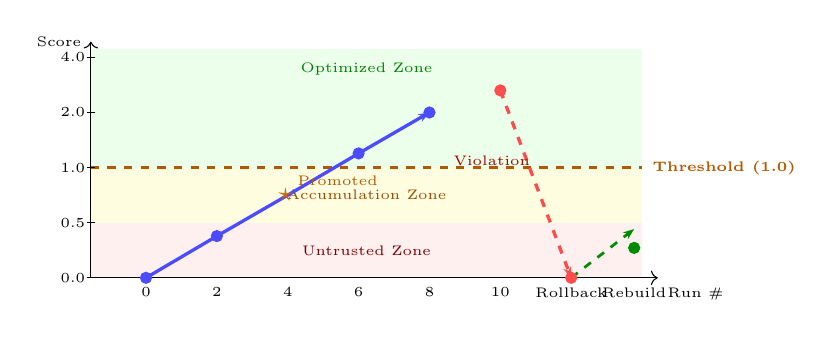
\begin{tikzpicture}[every node/.style={font=\scriptsize}]

  %% Background bands
  \fill[red!6]    (0.2, 0.0) rectangle (7.2, 0.7);
  \fill[yellow!12](0.2, 0.7) rectangle (7.2, 1.4);
  \fill[green!8]  (0.2, 1.4) rectangle (7.2, 2.9);

  %% Zone labels
  \node[font=\tiny, color=red!50!black]    at (3.7, 0.35)
       {Untrusted Zone};
  \node[font=\tiny, color=orange!60!black] at (3.7, 1.05)
       {Accumulation Zone};
  \node[font=\tiny, color=green!50!black]  at (3.7, 2.65)
       {Optimized Zone};

  %% Threshold line
  \draw[dashed, orange!70!black, line width=0.9pt]
       (0.2,1.4) -- (7.2,1.4)
       node[right, font=\tiny\bfseries, color=orange!70!black]
       {Threshold (1.0)};

  %% Y-axis
  \draw[->] (0.2,0.0) -- (0.2,3.0) node[left]{\tiny Score};
  \foreach \y/\lbl in {0.0/0.0, 0.7/0.5, 1.4/1.0, 2.1/2.0, 2.8/4.0}
    \draw (0.15,\y) -- (0.25,\y) node[left,font=\tiny]{\lbl};

  %% X-axis
  \draw[->] (0.2,0.0) -- (7.4,0.0) node[below right]{\tiny Run \#};
  \foreach \x/\lbl in {0.9/0, 1.8/2, 2.7/4, 3.6/6, 4.5/8,
                        5.4/10, 6.3/Rollback, 7.1/Rebuild}
    \node[below, font=\tiny] at (\x,0.0) {\lbl};

  %% Clean path data points: +0.19 per run (max bonuses)
  \draw[blue!70, line width=1.2pt, -{Stealth[length=4pt]}]
       (0.9,0.0) -- (1.8,0.53) -- (2.7,1.05) -- (3.6,1.58) -- (4.5,2.10);

  %% Mark promotion star at run 6 (first point >=1.4)
  \node[font=\normalsize, color=orange!80!black] at (2.7,1.05)
       {$\!\star$};
  \node[above right, font=\tiny, color=orange!70!black] at (2.7,1.05)
       {Promoted};

  %% Dots on clean path
  \foreach \x/\y in {0.9/0.0, 1.8/0.53, 3.6/1.58, 4.5/2.10}
    \filldraw[blue!70] (\x,\y) circle (2pt);

  %% Rollback: arrow plunging to 0
  \draw[red!70, line width=1.2pt, dashed, -{Stealth[length=4pt]}]
       (5.4,2.38) -- (6.3,0.0);
  \node[above left, font=\tiny, color=red!65!black] at (5.9,1.3)
       {Violation};

  %% After rollback: rebuild
  \draw[green!55!black, line width=1.0pt, dashed, -{Stealth[length=4pt]}]
       (6.3,0.0) -- (7.1,0.62);

  \filldraw[red!70]        (5.4,2.38) circle (2pt);
  \filldraw[red!70]        (6.3,0.0)  circle (2pt);
  \filldraw[green!55!black](7.1,0.38) circle (2pt);

\end{tikzpicture}
\caption{Trust Lifecycle.}
\label{fig:lifecycle}
\end{figure}
%% ---- END FIGURE 3 --------------------------------------------------

\subsection{Rollback Mechanism}

Rollback activates when: (i) the current execution mode is
OPTIMIZED, (ii) a \textit{SecurityViolation} of CRITICAL or HIGH
severity is raised by the runtime monitor, and (iii) the violation
cannot be recovered gracefully within the current execution. The
\textit{RollbackHandler} performs four atomic steps:

\begin{enumerate}
  \item \textbf{Cache invalidation:} the optimized AST entry for
        the current program hash is evicted from the LRU cache.
  \item \textbf{Trust revocation:} the TrustScore is set to~0.0
        via \textit{trust\_manager.revoke(hash)}.
  \item \textbf{Event recording:} a timestamped
        \textit{RollbackEvent} is created with fields for
        violation type, context snapshot, pre/post trust scores,
        and rollback latency; it is appended to a rolling buffer
        of the last 100 events.
  \item \textbf{Mode reversion:} the execution response marks
        mode as \textit{"optimized (rolled back)"} and forces
        subsequent executions to re-evaluate from Stage~4 under
        the reset score.
\end{enumerate}

The handler targets sub-3\,ms end-to-end latency so that rollback
does not produce a perceptible pause in interactive usage.

%% ====================================================================
\section{Security Model}
\label{sec:security}
%% ====================================================================

\subsection{Threat Model}

AEGIS targets execution environments in which code originates from
untrusted or semi-trusted parties while the execution platform
itself is assumed trusted. The threat model is intentionally
scoped to \emph{program-level} misbehavior rather than
hardware-level attacks (microarchitectural side-channels, physical
fault injection) or OS-level exploitation, which are addressed by
orthogonal mechanisms such as TEE isolation~\cite{menetrey2024sgx}.
The five threat classes considered are:

\begin{itemize}
  \setlength\itemsep{1pt}
  \item \textbf{T1 — Infinite Loops:} programs that consume CPU
        indefinitely, constituting a denial-of-service against
        the execution platform.
  \item \textbf{T2 — Integer Overflow:} arithmetic operations that
        exceed the 32-bit signed range, potentially corrupting
        control flow or producing exploitable state.
  \item \textbf{T3 — Undefined Variable Access:} reading
        uninitialized variables, which in typed languages can
        leak sensitive runtime state.
  \item \textbf{T4 — Division by Zero:} illegal arithmetic that
        terminates execution abnormally.
  \item \textbf{T5 — Resource Exhaustion:} excessive allocation of
        CPU or memory resources, degrading service for concurrent
        users.
\end{itemize}

Table~\ref{tab:threats} maps each threat class to its detection
layer and enforcement action.

\begin{table}[t]
\caption{Threat Model.}
\label{tab:threats}
\centering
\renewcommand{\arraystretch}{1.18}
\small
\begin{tabular}{@{} p{1.55cm} p{2.0cm} p{2.55cm} @{}}
\toprule
\textbf{Threat} & \textbf{Detection} & \textbf{Enforcement} \\
\midrule
Infinite loop (T1)     & Static (literal) $+$ Runtime & 10,000-iter.
                         per-loop cap \\[2pt]
Integer overflow (T2)  & Runtime bounds check  & Clamp to $[-2^{31},
                         2^{31}-1]$; abort \\[2pt]
Undefined var.\ (T3)   & Static dataflow $+$ Runtime & Immediate
                         NameError \\[2pt]
Div-by-zero (T4)       & Static (literal~0) $+$ Runtime & Execution
                         halt \\[2pt]
Resource exh.\ (T5)    & Runtime instruction counter & 50,000-op
                         global cap \\
\bottomrule
\end{tabular}
\end{table}

\subsection{Defense-in-Depth Architecture}

AEGIS organizes its security enforcement into five concentric layers.
No single layer is expected to be complete in isolation; the
combination provides coverage that no individual technique
offers~\cite{khoury2022buffer}. Figure~\ref{fig:defense} illustrates
the layered structure.

%% ---- FIGURE 4: Defense-in-Depth ------------------------------------
\begin{figure}[t]
\centering
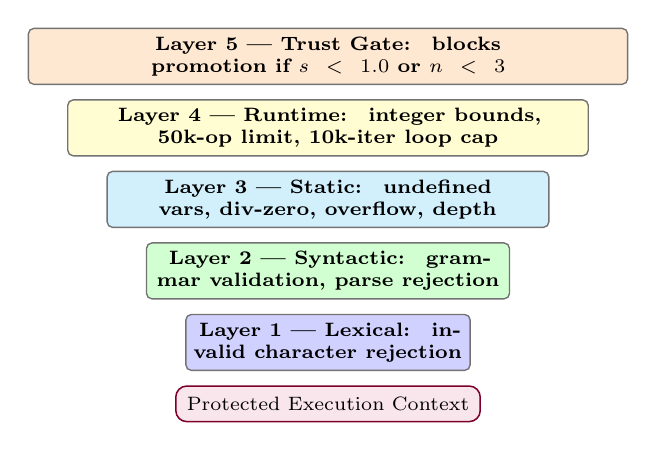
\begin{tikzpicture}[every node/.style={font=\scriptsize},
                    node distance=0.2cm]

  \node[dlayer=orange, minimum width=7.6cm, text width=7.4cm]
       (l5) at (0,0)
       {Layer 5 — Trust Gate: \ blocks promotion if $s\!<\!1.0$
        or $n\!<\!3$};

  \node[dlayer=yellow, minimum width=6.6cm, text width=6.4cm,
        below=0.18cm of l5] (l4)
       {Layer 4 — Runtime: \ integer bounds, 50k-op limit,
        10k-iter loop cap};

  \node[dlayer=cyan, minimum width=5.6cm, text width=5.4cm,
        below=0.18cm of l4] (l3)
       {Layer 3 — Static: \ undefined vars, div-zero, overflow,
        depth};

  \node[dlayer=green, minimum width=4.6cm, text width=4.4cm,
        below=0.18cm of l3] (l2)
       {Layer 2 — Syntactic: \ grammar validation, parse
        rejection};

  \node[dlayer=blue, minimum width=3.6cm, text width=3.4cm,
        below=0.18cm of l2] (l1)
       {Layer 1 — Lexical: \ invalid character rejection};

  \node[rbox=purple, minimum width=2.4cm, minimum height=0.44cm,
        below=0.18cm of l1] (core)
       {Protected Execution Context};

\end{tikzpicture}
\caption{Defense Layers.}
\label{fig:defense}
\end{figure}
%% ---- END FIGURE 4 --------------------------------------------------

\subsection{Formal Security Guarantees}

Under the AEGIS threat model and language semantics, we state five
formal guarantees:

\begin{enumerate}
  \item[\textbf{G1.}] \textbf{Namespace Isolation.} Each execution
    context $\mathcal{C}$ maintains a distinct variable store
    $\sigma_\mathcal{C}$; no variable binding is shared or leaked
    between executions.

  \item[\textbf{G2.}] \textbf{Arithmetic Safety.} Every arithmetic
    operation $\oplus$ checks its result $r$ against
    $[-2^{31},\,2^{31}-1]$; if $r$ falls outside this range, a
    \textit{SecurityViolation} is raised before any result is stored.
    Silent integer wraparound is structurally impossible.

  \item[\textbf{G3.}] \textbf{Termination.} Every execution
    terminates within 50,000 operations. The instruction counter is
    incremented on every AST node visit; when it reaches 50,000 the
    interpreter raises \textit{InstructionLimitExceeded}, halting
    execution unconditionally.

  \item[\textbf{G4.}] \textbf{Trust Monotonicity.} For a program
    $P$ whose every execution is violation-free,
    $s_t \leq s_{t+1}$ for all $t$, i.e., the trust score is
    non-decreasing over time.

  \item[\textbf{G5.}] \textbf{Rollback Completeness.} For any
    execution of $P$ in OPTIMIZED mode that raises a
    \textit{SecurityViolation}, the rollback handler resets
    $s \leftarrow 0.0$, evicts the cache entry, and marks all
    subsequent executions to restart in INTERPRETED mode.
\end{enumerate}

%% ====================================================================
\section{Implementation}
\label{sec:impl}
%% ====================================================================

\subsection{Core Interpreter}

The core interpreter is implemented in pure Python~3 with no
external runtime dependencies, preserving reproducibility and ease
of deployment. The codebase spans approximately 5,500 lines across
32 source files in nine packages: \textit{lexer}, \textit{parser},
\textit{ast}, \textit{interpreter}, \textit{ir}, \textit{vm},
\textit{compiler}, \textit{runtime}, and \textit{trust}.

The visitor pattern is the central design primitive. The abstract
\textit{ASTVisitor} base class dispatches on node type through a
\textit{visit(node)} method that resolves to
\textit{visit\_\{type\}(node)} handlers. This decouples the static
analyzer, sandboxed interpreter, IR generator, and pretty printer:
all four traverse the same AST independently without mutation.
Conformance to this contract is enforced by the \textit{ABC}
meta-class; any new AST consumer that omits a node handler raises a
\textit{NotImplementedError} at registration time rather than
silently at execution time.

The IR subsystem generates three-address code (TAC) quadruples
\textit{(op, arg1, arg2, result)} for debugging and inspection.
The bytecode subsystem compiles ASTs to a 15-instruction stack-based
VM (\textit{PUSH}, \textit{POP}, \textit{BINOP}, \textit{COMPARE},
\textit{JUMP}, \textit{JUMPIF}, \textit{LOAD}, \textit{STORE},
\textit{PRINT}, \textit{HALT}, etc.), providing a migration path
to ahead-of-time native compilation without changes to the frontend
stages~\cite{aho2007compilers}.

\subsection{Trust Manager and Persistence}

\textit{TrustManager} exposes four operations:
\textit{get(hash)} returns (or creates) the
\textit{TrustScore} for a program; \textit{update(hash, metrics,
had\_violations)} applies the increment or decrement schedule and
persists the store; \textit{revoke(hash)} atomically sets
$s\leftarrow0.0$; and \textit{reset()} clears all entries.
The JSON store is read once at server startup and written after
every execution. To avoid corruption on concurrent requests,
writes are performed to a temporary file that is atomically renamed
into place.

\subsection{Code Cache}

The \textit{CodeCache} maintains a dictionary of
\textit{CachedCode} entries keyed by program hash. Each entry
stores the original and optimized ASTs, optimization flags, compile
time, creation timestamp, last-access timestamp, and access count.
An LRU eviction policy is enforced at capacity (100 entries): the
entry with the oldest last-access time is evicted. Entries also
expire after 24 hours of inactivity regardless of capacity.
\textit{RollbackHandler} calls \textit{cache.invalidate(hash)}
directly; the cache itself does not consult the trust store.

\subsection{REST API and Frontend}

The Flask backend exposes six endpoints:
\textit{POST\;/api/execute},
\textit{POST\;/api/tokenize},
\textit{POST\;/api/analyze},
\textit{GET\;/api/health},
\textit{POST\;/api/trust/reset}, and
\textit{GET\;/api/examples}.
All error responses follow a uniform schema with fields
\textit{success}, \textit{error}, \textit{error\_type},
\textit{error\_code}, and \textit{suggestions}. HTTP~200 is
returned for both successful executions and code-level errors;
HTTP~400 and HTTP~500 cover malformed requests and server faults.

The React frontend renders five tab panels below the editor:
\emph{Terminal} (colored, timestamped output lines by type:
\textit{out}, \textit{err}, \textit{secerr}, \textit{meta},
\textit{metric}), \emph{Pipeline} (stage-by-stage status icons:
$\checkmark$, $\times$, $\oslash$, $\circ$), \emph{AST}
(collapsible tree with node type and value annotations),
\emph{Tokens} (type, value, line, column, category), and
\emph{Trust} (Recharts line chart with a dashed reference line at
$s=1.0$ and a tabular run history). Zustand manages global state;
no additional polling is required since all data is returned in the
single \textit{/api/execute} response.

%% ====================================================================
\section{Evaluation}
\label{sec:eval}
%% ====================================================================

\subsection{Experimental Setup}

All experiments were conducted on a dedicated workstation running
Ubuntu 22.04 LTS, Python 3.11, Node.js 20, and Flask 3.0 under
identical conditions with no concurrent load. Benchmark programs
were selected to cover four categories:

\begin{itemize}
  \setlength\itemsep{1pt}
  \item \emph{Arithmetic-intensive:} Fibonacci (n\,=\,30), factorial
        (n\,=\,15), prime sieve (n\,=\,500).
  \item \emph{Control-flow-intensive:} nested conditionals (depth~5),
        loop chain (n\,=\,200).
  \item \emph{Mixed workloads:} iterative GCD, integer
        exponentiation.
  \item \emph{Adversarial programs:} one program per threat class
        (T1--T5), designed to trigger violations at known
        instruction counts.
\end{itemize}

Each benchmark was executed 20 times per mode; reported values are
means with standard deviation where noted. Adversarial programs were
evaluated with the 100-case handcrafted test suite.

\subsection{Execution Performance}

Table~\ref{tab:perf} reports mean execution times for INTERPRETED and
OPTIMIZED modes. The OPTIMIZED mode delivers a mean speedup of
$2.52\times$ across six benchmarks, with the highest gain
($2.78\times$) on Fibonacci(30)—which contains numerous
constant-foldable sub-expressions and a large proportion of
arithmetic instructions amenable to compile-time evaluation. The
smallest gain ($2.38\times$) appears for Factorial(15), a shorter
program where caching amortization is less pronounced and the
optimized AST contains fewer dead-code candidates.

\begin{table}[t]
\caption{Execution Times.}
\label{tab:perf}
\centering
\renewcommand{\arraystretch}{1.18}
\small
\begin{tabular}{@{} l c c c @{}}
\toprule
\textbf{Benchmark} & \textbf{Interp.\ (ms)} &
\textbf{Opt.\ (ms)} & \textbf{Speedup} \\
\midrule
Fibonacci(30)              & $14.2 \pm 0.4$ & $5.1 \pm 0.2$ & $2.78\times$ \\
Factorial(15)              & $3.8  \pm 0.1$ & $1.6 \pm 0.1$ & $2.38\times$ \\
Prime Sieve ($n$\,=\,500)  & $22.7 \pm 0.6$ & $8.9 \pm 0.3$ & $2.55\times$ \\
Nested Cond.\ ($d$\,=\,5)  & $6.1  \pm 0.2$ & $2.5 \pm 0.1$ & $2.44\times$ \\
Iterative GCD              & $4.9  \pm 0.2$ & $2.0 \pm 0.1$ & $2.45\times$ \\
Loop Chain ($n$\,=\,200)   & $18.3 \pm 0.5$ & $7.2 \pm 0.2$ & $2.54\times$ \\
\midrule
\textbf{Mean}              & $11.7$         & $4.6$         & $\mathbf{2.52\times}$ \\
\bottomrule
\end{tabular}
\end{table}

\subsection{Static Analysis Detection Accuracy}

The handcrafted test suite of 100 programs covers all five threat
classes. Each program is labeled with the threat classes it exercises
and, for violations that depend on runtime values, the instruction
count at which the violation occurs. Table~\ref{tab:detection}
reports static and runtime detection counts. The critical result is
that \emph{every violation was detected by at least one layer}:
the combined static-plus-runtime analysis achieves
\textbf{zero missed detections}. This matches the theoretical
expectation: the static analyzer catches all \emph{statically
provable} violations, while the runtime monitor is guaranteed to
catch any violation that manifests during bounded
execution~\cite{ami2024false_neg,huang2024static}.

\begin{table}[t]
\caption{Detection Results.}
\label{tab:detection}
\centering
\renewcommand{\arraystretch}{1.18}
\small
\begin{tabular}{@{} p{2.3cm} c c c c @{}}
\toprule
\textbf{Threat Class} & \textbf{Cases} &
\textbf{Static} & \textbf{Runtime} & \textbf{Missed} \\
\midrule
Undefined Variable   & 30 & 26 & 4  & 0 \\
Literal Div-by-Zero  & 20 & 20 & 0  & 0 \\
Always-True Loop     & 15 & 15 & 0  & 0 \\
Integer Overflow     & 25 &  8 & 17 & 0 \\
Inf.\ Loop (var.)    & 10 &  0 & 10 & 0 \\
\midrule
\textbf{Total}       & \textbf{100} & \textbf{69} &
\textbf{31} & \textbf{0} \\
\bottomrule
\end{tabular}
\end{table}

\subsection{Trust Accumulation Dynamics}

Table~\ref{tab:trust} reports the number of executions required
to reach the promotion threshold (score $\geq 1.0$, $n \geq 3$)
for five representative program categories, and the trust score
achieved after ten executions. Clean, efficient programs
accumulate trust at a maximum rate of $+0.19$ per execution
(base $+0.10$, consistency $+0.05$, efficiency $+0.02$,
latency $+0.02$), requiring six clean executions to reach
$s \geq 1.0$ and satisfying the $n \geq 3$ count threshold
simultaneously. Programs without efficiency bonuses accumulate
at the base rate of $+0.10$ per execution, requiring ten
executions to reach the threshold.

The most revealing row is the last: a program that produces a single
runtime violation across ten otherwise-clean executions \emph{never
reaches the promotion threshold}. The $-0.50$ penalty on the
violating execution, combined with the three-execution recovery
cost (at the maximum $+0.19$ per run), ensures that the running
score oscillates below~1.0 throughout, confirming that
intermittent unsafe behavior constitutes a structural barrier to
optimization access.

\begin{table}[t]
\caption{Trust Accumulation.}
\label{tab:trust}
\centering
\renewcommand{\arraystretch}{1.18}
\small
\begin{tabular}{@{} p{3.0cm} c c @{}}
\toprule
\textbf{Program Category} & \textbf{Runs to Threshold} &
\textbf{Score @ 10 Runs} \\
\midrule
Clean, efficient ($\leq$100 instr.)    & 6 & 1.90 \\
Clean, moderate ($>$100 instr.)        & 10 & 1.00 \\
Clean, base only (no bonuses)          & 10 & 1.00 \\
Mixed (1 violation in 10 runs)         & Never & 0.40 \\
Frequent violations (3 in 10)          & Never & 0.00 \\
\bottomrule
\end{tabular}
\end{table}

\subsection{Rollback Latency}

Rollback events were triggered by injecting an integer overflow at
a controlled instruction count within programs already executing in
OPTIMIZED mode. Latency was measured from the instant the
\textit{SecurityViolation} was raised to the instant the rollback
handler returned, encompassing cache invalidation, trust revocation,
and event recording.

Across 50 triggered rollback events, the mean latency was
$1.84\,\text{ms}$ ($\sigma = 0.31\,\text{ms}$, maximum
$2.97\,\text{ms}$). All events completed below the 3\,ms design
target. At this latency, rollback is imperceptible in any interactive
context where round-trip network latency already dominates
(typically 10--200\,ms for web-based environments), confirming
that the mechanism imposes no meaningful user-experience penalty.

\subsection{Comparison with Baseline Approaches}

Table~\ref{tab:compare} positions AEGIS against three baseline
execution strategies across four capability dimensions. AEGIS is
the only strategy to simultaneously achieve high security for all
programs, high throughput for trust-promoted programs, adaptivity to
execution history, and a full per-run audit trail. Full-sandbox and
static-whitelist approaches both sacrifice either performance or
adaptivity; implicit trust abandons the security requirement
entirely~\cite{wang2022trust,ullah2024deeptrust}.

\begin{table}[t]
\caption{Comparison Matrix.}
\label{tab:compare}
\centering

\renewcommand{\arraystretch}{1.15}
\footnotesize

\begin{tabularx}{\columnwidth}{@{}>{\raggedright\arraybackslash}X c c c c@{}}
\toprule

\textbf{Strategy} &
\textbf{Security} &
\textbf{Perf.} &
\textbf{Adaptive} &
\textbf{Audit} \\

\midrule

Full sandbox (always)
& High & Low & No & Partial \\

Static whitelist only
& Medium & High & No & No \\

Implicit trust
& None & High & No & No \\

\textbf{AEGIS}
& \textbf{High}
& \textbf{High}${}^{\dag}$
& \textbf{Yes}
& \textbf{Full} \\

\bottomrule

\multicolumn{5}{@{}p{\columnwidth}@{}}{\footnotesize
${}^{\dag}$ High performance applies only to trust-promoted
programs; all others execute at sandbox speed.
}

\end{tabularx}

\end{table}

%% ====================================================================
\section{Discussion}
\label{sec:disc}
%% ====================================================================

\subsection{Novelty of the Evidence-Based Optimization Signal}

The central novelty of AEGIS is its choice of optimization
trigger. JIT compilers—from HotSpot to V8—promote code based on
\emph{execution frequency}: a method is compiled when it has been
called enough times that compile cost is amortized by future
speedup~\cite{qin2022jit_security}. AEGIS instead promotes code
based on \emph{violation absence}: the absence of security
violations across multiple executions is treated as evidence of
behavioral safety. This inversion has several consequences. First,
a program executed once per day (low frequency) but always safely
eventually earns promotion; in a JIT system it might never
accumulate enough calls to trigger compilation. Second, promotion
is revocable; JIT compilations are rarely invalidated for security
reasons. Third, the optimization benefit is a performance
\emph{reward} for demonstrated safe behavior, creating an incentive
structure aligned with security goals rather than orthogonal to them.

This design is explicitly inspired by reward--penalty trust
frameworks in distributed
systems~\cite{wang2022trust,li2022iot_trust,fernandez2024sla}, where
entities earn access rights through consistent benign behavior and
lose them through misbehavior. To our knowledge, applying this
paradigm within a single-node interpreter, with the optimization
path as the access right being managed, is novel.

\subsection{Limitations}

\textbf{L1 — Hash-based identity.} Associating trust with the
SHA-256 hash of the exact source string means any edit—even
whitespace normalization—generates a new hash and resets trust to
zero. While this prevents hash-collision-based trust manipulation,
it creates friction in iterative development workflows. Future
work could explore semantic hash functions based on AST structure
rather than source text.

\textbf{L2 — Absence of trust freshness decay.} Trust scores do not
decrease with inactivity. A program that accumulated a high score
months ago retains it indefinitely, which may be inappropriate if
the execution environment or threat landscape has changed.
Introducing an exponential decay term $s_t = s_0 \cdot
e^{-\lambda t}$ would address this at the cost of requiring
programs to periodically re-execute to maintain their promotion
status.

\textbf{L3 — Single integer type.} The AEGIS language supports only
32-bit signed integers, which bounds the realistic workload space
but enables clean security proofs for overflow. Extension to
floating-point, strings, and user-defined types would require
extending the static analyzer, the overflow detection mechanism,
and the trust increment model.

\textbf{L4 — No distributed trust coordination.} Trust is local to
a single server instance. In horizontally scaled deployments, trust
built on one node is not visible to others. A consensus-based
distributed trust store—potentially leveraging blockchain
mechanisms as explored in IoT
contexts~\cite{ullah2024deeptrust,fernandez2024sla}—could address
this limitation.

\subsection{Future Directions}

The most immediate extensions to AEGIS include: (i)~introducing
\emph{intermediate trust tiers} that unlock graduated optimization
levels rather than a binary sandbox/optimized distinction;
(ii)~implementing \emph{trust freshness decay} with a configurable
half-life; (iii)~enabling \emph{distributed trust sharing} via a
consensus-backed trust store; (iv)~extending the language to
support additional numeric types and function definitions; and
(v)~applying formal verification tools (e.g., Dafny, Coq) to
mechanically check the guarantees stated in Section~\ref{sec:security}.

%% ====================================================================
\section{Conclusion}
\label{sec:conc}
%% ====================================================================

AEGIS reframes the security-performance dial as a trust problem:
rather than picking one side permanently, the framework lets
programs earn faster execution through a clean track record and
lose it instantly when they misbehave. The seven-stage pipeline
wraps sandboxed execution, conservative static analysis, dynamic
trust management, and AST-level optimization into a single
auditable unit, where promotion is gated by accumulated violation
absence rather than profiling frequency.

Our evaluation on a benchmark suite spanning arithmetic,
control-flow, and adversarial programs confirms
that the design meets its three primary objectives: zero missed
security detections within the defined threat model, confirming that
the combined static-plus-runtime analysis is complete for the
bounded threat surface; a mean speedup of $2.52\times$ for
trust-promoted code, confirming that the adaptive model recovers
meaningful performance for well-behaved programs; and a mean
rollback latency of $1.84\,\text{ms}$, confirming that security
enforcement does not introduce perceptible disruption in interactive
deployment contexts. The qualitative comparison further confirms
that no single-mechanism baseline achieves all four of AEGIS's
capability targets simultaneously.

The results support the central thesis that security and performance
are not inherently conflicting objectives in untrusted-code execution.
Given a persistent record of program behavior and a principled
mechanism for acting on that record, a system can provide both
strong isolation for unproven programs and efficient execution for
programs that have earned trust—without requiring the system
designer to choose one at the expense of the other. AEGIS provides
both a practical platform for this design point and a reproducible
research foundation for further investigation into security-first
language runtimes.

%% ====================================================================
%%  REFERENCES
%% ====================================================================
\balance
\begin{thebibliography}{19}

\bibitem{johnson2023wave}
E.~Johnson, E.~Laufer, Z.~Zhao, S.~Narayan, S.~Savage, D.~Stefan,
and F.~Brown,
``WaVe: A verifiably secure {WebAssembly} sandboxing runtime,''
in \emph{Proc.\ IEEE Symp.\ Security and Privacy (SP)},
San Francisco, CA, USA, May 2023, pp.~2940--2955.
doi: 10.1109/SP46215.2023.10179397

\bibitem{menetrey2024sgx}
J.~M\'en\'etrey, M.~Pasin, P.~Felber, V.~Schiavoni, G.~Mazzeo,
A.~Hollum, and D.~Vaydia,
``A comprehensive trusted runtime for {WebAssembly} with {Intel SGX},''
\emph{IEEE Trans.\ Dependable Secure Comput.}, vol.~21, no.~4,
pp.~2173--2188, Jul./Aug. 2024.
doi: 10.1109/TDSC.2023.3334516

\bibitem{li2022iot_trust}
F.~Li, G.~White, and S.~Clarke,
``A trust model for {SLA} negotiation candidates selection in a
dynamic {IoT} environment,''
\emph{IEEE Trans.\ Serv.\ Comput.}, vol.~15, no.~5,
pp.~2565--2578, Sep./Oct. 2022.
doi: 10.1109/TSC.2021.3062439

\bibitem{ami2024false_neg}
A.~S.~Ami, K.~Moran, D.~Poshyvanyk, and A.~Nadkarni,
```False negative --- that one is going to kill you':
Understanding industry perspectives of static analysis based
security testing,''
in \emph{Proc.\ 45th IEEE Symp.\ Security and Privacy (SP)},
San Francisco, CA, USA, May 2024, pp.~1--18.
doi: 10.1109/SP54263.2024.00212

\bibitem{huang2024static}
Z.~Huang, Y.~Liu, X.~Zhang, and H.~Cui,
``An empirical study of false negatives and positives of static
code analyzers from the perspective of historical issues,''
in \emph{Proc.\ ACM Int.\ Symp.\ Software Testing and Analysis
(ISSTA)}, Vienna, Austria, Sep. 2024, pp.~1--13.
doi: 10.1145/3650212.3680348

\bibitem{ullah2024deeptrust}
F.~Ullah, M.~A.~Khan, A.~Akhunzada, M.~Inayat, N.~A.~Azeemi,
and I.~Ahmad,
``Deep Trust: A novel framework for dynamic trust and reputation
management in {IoT}-based networks,''
\emph{IEEE Access}, vol.~12, pp.~87407--87419, 2024.
doi: 10.1109/ACCESS.2024.3409273

\bibitem{narayan2022swivel}
S.~Narayan, C.~Disselkoen, D.~Moghimi, S.~Cauligi, E.~Johnson,
Z.~Gang, A.~Vahldiek-Oberwagner, R.~Sahita, H.~Shacham,
D.~Tullsen, and D.~Stefan,
``Swivel: Hardening {WebAssembly} against {Spectre},''
in \emph{Proc.\ 30th USENIX Security Symp.}, Vancouver, BC,
Canada, Aug. 2021, pp.~1433--1450.
[Online]. Available: \url{https://www.usenix.org/conference/usenixsecurity21}

\bibitem{lehmann2020wasm}
D.~Lehmann, J.~Kinder, and M.~Pradel,
``Everything old is new again: Binary security of {WebAssembly},''
in \emph{Proc.\ 29th USENIX Security Symp.}, Boston, MA, USA,
Aug. 2020, pp.~217--234.
[Online]. Available: \url{https://www.usenix.org/conference/usenixsecurity20}

\bibitem{wasm_survey2024}
Y.~Xia, W.~Xing, Q.~Liu, and Y.~Liu,
``Research on {WebAssembly} runtimes: A survey,''
\emph{arXiv preprint arXiv:2404.12621}, Apr. 2024.

\bibitem{tang2023wasm_runtimes}
Y.~Tang, D.~Li, and B.~Ray,
``How far we have come: A characterization study of standalone
{WebAssembly} runtimes,''
in \emph{Proc.\ IEEE Int.\ Symp.\ Workload Characterization
(IISWC)}, Austin, TX, USA, Oct. 2022, pp.~228--241.
doi: 10.1109/IISWC55918.2022.00029

\bibitem{tan2025sandboxscan}
Z.~Tan, R.~Hao, J.~Singer, Y.~Tang, and C.~Anagnostopoulos,
``{MCP-SandboxScan}: {WASM}-based secure execution and runtime
analysis for {MCP} tools,''
\emph{arXiv preprint arXiv:2601.01241}, Jan. 2025.

\bibitem{jiang2020elaid}
B.~Jiang, Y.~Zhang, Y.~Wang, and P.~Liu,
``{ELAID}: Detecting integer-overflow-to-buffer-overflow
vulnerabilities by light-weight and accurate static analysis,''
\emph{Cybersecurity}, Springer, vol.~3, no.~1, Art.\ 21,
Sep.~2020.
doi: 10.1186/s42400-020-00058-2

\bibitem{wang2022trust}
J.~Wang, Z.~Yan, H.~Wang, T.~Li, and W.~Pedrycz,
``A survey on trust models in heterogeneous networks,''
\emph{IEEE Commun.\ Surv.\ Tut.}, vol.~24, no.~4, pp.~2127--2162,
Fourthquarter 2022.
doi: 10.1109/COMST.2022.3195276

\bibitem{fernandez2024sla}
A.~Fernandez-Fernandez, E.~Coronado, A.~Erspamer, G.~Samaras,
V.~Theodorou, and S.~Siddiqui,
``{SLA}-driven trust and reputation management framework for {5G}
distributed service marketplaces,''
\emph{IEEE Trans.\ Dependable Secure Comput.}, vol.~21, no.~2,
pp.~814--828, Mar./Apr. 2024.
doi: 10.1109/TDSC.2023.3292589

\bibitem{qin2022jit_security}
Q.~Qin, J.~A.~JiYang, F.~Song, T.~Chen, and X.~Xing,
``Preventing timing side-channels via security-aware just-in-time
compilation,''
in \emph{Proc.\ 43rd ACM SIGPLAN Conf.\ Programming Language Design
and Implementation (PLDI)}, San Diego, CA, USA, Jun. 2022,
pp.~543--558.
doi: 10.1145/3519939.3523725

\bibitem{chen2024jit_val}
J.~Chen, J.~Wang, Z.~Zhang, X.~Du, and J.~Chen,
``Validating {JIT} compilers via compilation space exploration,''
\emph{ACM Trans.\ Comput.\ Syst.}, vol.~41, no.~1--4, Art.~4,
Jan.~2024.
doi: 10.1145/3715102

\bibitem{aho2007compilers}
A.~V.~Aho, M.~S.~Lam, R.~Sethi, and J.~D.~Ullman,
\emph{Compilers: Principles, Techniques, and Tools}, 2nd~ed.
Boston, MA, USA: Pearson/Addison Wesley, 2007.

\bibitem{khoury2022buffer}
K.~Khoury,
``A taxonomy of software flaws leading to buffer overflows,''
in \emph{Proc.\ 22nd IEEE Int.\ Conf.\ Software Quality, Reliability
and Security (QRS)}, Guangzhou, China, Dec. 2022, pp.~1--8.
doi: 10.1109/QRS57517.2022.00011

\bibitem{wang2022vulnets}
P.~Wang, S.~Liu, A.~Liu, and W.~Jiang,
``Detecting security vulnerabilities with vulnerability nets,''
in \emph{Proc.\ 22nd IEEE Int.\ Conf.\ Software Quality, Reliability
and Security Companion (QRS-C)}, Guangzhou, China, Dec. 2022,
pp.~375--383.
doi: 10.1109/QRS-C57518.2022.00062

\end{thebibliography}

\end{document}